\documentclass{juliacon}
\setcounter{page}{1}

\begin{document}

% **************GENERATED FILE, DO NOT EDIT**************

\title{My JuliaCon proceeding}

\author[1]{Jacob S. Zelko}
\author[1, 2]{Malina Hy}
\author[1, 2]{Varshini Chinta}
\affil[1]{Georgia Tech Research Institute}
\affil[2]{Georgia Institute of Technology}

\keywords{Observational Health, OMOP Common Data Model, Database Management, Characterization}

\hypersetup{
pdftitle = {My JuliaCon proceeding},
pdfsubject = {JuliaCon 2019 Proceedings},
pdfauthor = {Jacob S. Zelko, Malina Hy, Varshini Chinta},
pdfkeywords = {Observational Health, OMOP Common Data Model, Database Management, Characterization},
}



\maketitle

\begin{abstract}

Observational health continues to be a growing field in health informatics research as electronic health records (EHR), patient medical claims, and other ancilliary patient data source become more readily computable and accessible to researchers.
JuliaHealth is poised as an ecosystem to innovate within this area of research by bringing highly performant analytics approaches, composable solutions, and interoperable software that leverages prior state of the art. 
This paper will discuss the state of the art observational health research tools within the JuliaHealth ecosystem and how JuliaHealth is prepared to further research goals within this domain.

\end{abstract}

\section{Introduction}

Over the past $10$ years, there have been several innovations within the observational health research.
Arguably, the most crucial innovation that has emerged is the Observational Medical Outcomes Partnership Common Data Model (OMOP CDM) which was designed specifically to standardize observational health data to enable transferable analyses.
The importance of this model has become apparent within open science organizations like the OHDSI (Observational Health Data Science and Informatics) network where members across $100+$ countries with access to various health systems have been able to successfully map their patient data to the OMOP CDM.
This has led to successful collaboration relationships across countries where one research group can develop a network study and then disseminate the study across collaborators leading to the idea that you can "write once, run everywhere."

The OMOP CDM itself does not require a specific technology to work with the data stored in this standard.
It features a person-centric design where each domain records personal identity while prioritizing data protection through the limiting of information that could endanger patient anonymity.
As the OMOP CDM has become a cornerstone in running these widely distributed network studies, special attention to developing tools around handling OMOP CDM data is necessary to meaningfully contribute within the observational health research space.

\subsection{What Is JuliaHealth and Its Goals?}
JuliaHealth is an open-source organization under the umbrella of the Julia language. It leverages the high-performance of the Julia language in the health field while for example handling large data sets and manipulating them. JuliaHealth aims to be researchers' companion in making use of the observational-health data as Julia is easy to be learnt syntax-wise.

\subsection{Status of Conducting Observational Health Research in Julia}

Over the history of JuliaHealth, a sub-ecosystem within the JuliaHealth ecosystem has developed which is dedicated to performing observational health research around the OMOP CDM.
This sub-ecosystem is now mature enough to conduct internationally federated observational health research using tools housed within JuliaHealth and Julia exclusively.
Additionally, due to the strong interoperability capabilities of Julia, rather than forgoing or completely reinventing aspects of pre-existing observational health research tools, the Julia observational health subecosystem builds on some of these innovations.

As an example, OHDSI's HADES (Health Analytics Data-To-Evidence Suite) has been in existence for over $10$ years and has several rich packages.
One of the premier tools within HADES is the ATLAS Shiny application which was developed to "support the design and execution of observational analyses to generate real world evidence from patient level observational data."

\section{Describing an Observational Health Research Workflow Using JuliaHealth}

TODO: Discuss the "big idea" of what this workflow could look like

\subsection{Cohort Expressions Usability}

Broadly, ATLAS has become the de facto tool to develop patient phenotype definitions within observational health research contexts.
These phenotype definitions have varying levels of complexity where they can be very simple (finding all patients with one health condition or diagnosis) or grow to be extremely complex (defining controlled, uncontrolled, and indeterminate patient cohorts based on medications, lab results, etc.)
The computable phenotype definitions that ATLAS generates based on phenotype definitions are in a variety of serialization formats such as JSON (see \ref{appendix:json}) or prepared SQL expressions available in multiple SQL flavors (see \ref{appendix:postgresql}).

The Julia package, OHDSICohortExpressions.jl, exists specifically to ingest these serialized expressions of computable phenotype definitions and create patient cohorts that match the given criterion in the definition.
How this tool works is to 1) read and verify the serialized computable phenotype definition 2) reinterpret the serialization into the FunSQL.jl Domain Specific Language 3) return a prepared SQL statement against a given SQL database that queries an OMOP CDM database for the desired patient population(s) of interest.
Once these prepared statements are made, researchers can execute the generated SQL against their OMOP CDM instance to generate cohorts for future analyses.

\subsection{Fine-Grain Creation of Cohorts}

Although OHDSICohortExpressions.jl is sufficient to translate existing phenotype definitions generated in ATLAS to executable queries, oftentimes, there is a tricky problem of how to best iterate on phenotype definitions.
Often, one has to take an existing definition and either revise to a more narrow cohort or write manual code to build more niche cohorts after an initial definition is created.
This refactoring of a phenotype definition can lead to conflating ideas within conversation between expert clinical reviewers, analysts, and health researchers.
This broadly can be the notions of what we are exploring (the phenotype definition; often the responsibility of a clinical reviewer), what is possible to compute upon (the computable phenotype definition; often the responsibility of an analyst), and the goals of the overall study.
For situations such as these, the tool OMOPCDMCohortCreator.jl was created.

OMOPCDMCohortCreator.jl allows one to iteratively build a patient population quickly and easily.
One can use patient pools developed from pre-existing cohorts defined off of phenotype definitions as a starting point in exploring patients or create new patient populations quickly without the need for a well-defined phenotype definition.
This can enable analysts to more quickly understand what is inside their data assets, do "quick" analysis of a particular smaller research question, and enable a more distinct separation of work between a clinical expert reviewer and analyst teams.
It is highly recommended to still create phenotype definitions about particular populations one explores.

TODO: Add reference to phenotype paper
TODO: Add small example showing iterative process 
TODO: Reference capr somehow

\subsection{Working with Patient Databases}

One of the biggest styming factors within not only the Julia ecosystem, but observational health research in general has been the difficulty of working with different databases.
Although the OMOP CDM has been great for standardizing \textit{how} real world data is handled, there is a lack of consensus on \textit{what} is needed to handle these data assets.
For a variety of reasons, different groups will choose different database architectures (perhaps PostgreSQL for improved permission support, DuckDB for performance, or even SQLite for ease of use) but all are subtly different enough to create headaches in seamlessly working across different research sites.

The way that the Julia ecosystem handles this is via the creation of a common database interface called the DBInterface.
Specific Julia database packages can implement dispatches for this interace allowing users to have a much better experience working across databases.
In spite of the such benefits, for some users (and especially within the context of observational health studies), it can beneficial to have a more prescriptive interface where one just needs to pass perhaps a password, username, database name, and schema.
For that reason, we DBConnector.jl was created.

Although this is not an explicit JuliaHealth package, it was a pain point that was experienced throughout the process of observational health research across multiple partner sites.
The promise of DBConnector.jl is that with one line command, users can connect simply, and in a common (albeit opinionated) manner, to databases.
DBConnector unifies Julia database packages that implement the DBInterface to achieve this level of simplified connection making.

Finally, if someone needs more fine-grained control over a particular database connection, they can choose to eschew this package.
Instead, they can switch to the specific Julia database package that would give them the additional control.
Although they'll lose the simplicity of this package, core required functionality is not lost when working with databases.

TODO: Add database connector example
TODO: Reference database connector example
TODO: Reference that it was inspired by database connector OHDSI package
TODO: Mention package extensions utility

\subsection{Building on Current Tools and State of the Art}

TODO: Discuss OHDSIAPI.jl

\section{Conducting a Small-Scale Observational Health Research Study Using JuliaHealth Tools}

With the JuliaHealth tools that have now been created, we can now demonstrate an observational health study workflow that would be used in practice.
For this paper, we used two datasets: a synthetic patient dataset called \textit{Eunomia} and the MIMIC III patient dataset which had been converted into the OMOP CDM to illustrate the workflow provided by the Observational Health sub-ecosystem.
Reproducing the workflow using the \textit{Eunomia} dataset is made readily available at the repository here:

TODO: Add tutorial to separate repository
TODO: Create tutorial about Eunomia
TODO: Reference Eunomia

\textit{Eunomia} will be used to drive the workflow example looking at patients who have ever had a history of strep throat.
Results generated by the \textit{Eunomia} dataset will be shown for pedagogical purposes although the actual results of that analysis will be nonsensical given the synthetic nature of the database.
However, to complement this, a similar study will be done on the MIMIC III dataset characterizing individuals with a history of Type 2 Diabetes Mellitus to encourage discussion on what is practically possible with these tools.

\subsection{Connecting to a Database}

\begin{verbatim}
  import HealthSampleData: Eunomia
  import OMOPCDMCohortCreator as OCC

  eunomia = Eunomia()
  conn = DB(eunomia)

  occ.GenerateDatabaseDetails(
      :sqlite,
      "main"
  )

  occ.GenerateTables(conn)
\end{verbatim}

TODO: Replace with DBConnector syntax

\subsection{Bridging between OHDSI and JuliaHealth Communities}

Briding between tools used in the OHDSI and JuliaHealth communities is now exceptionally straightforward.

% 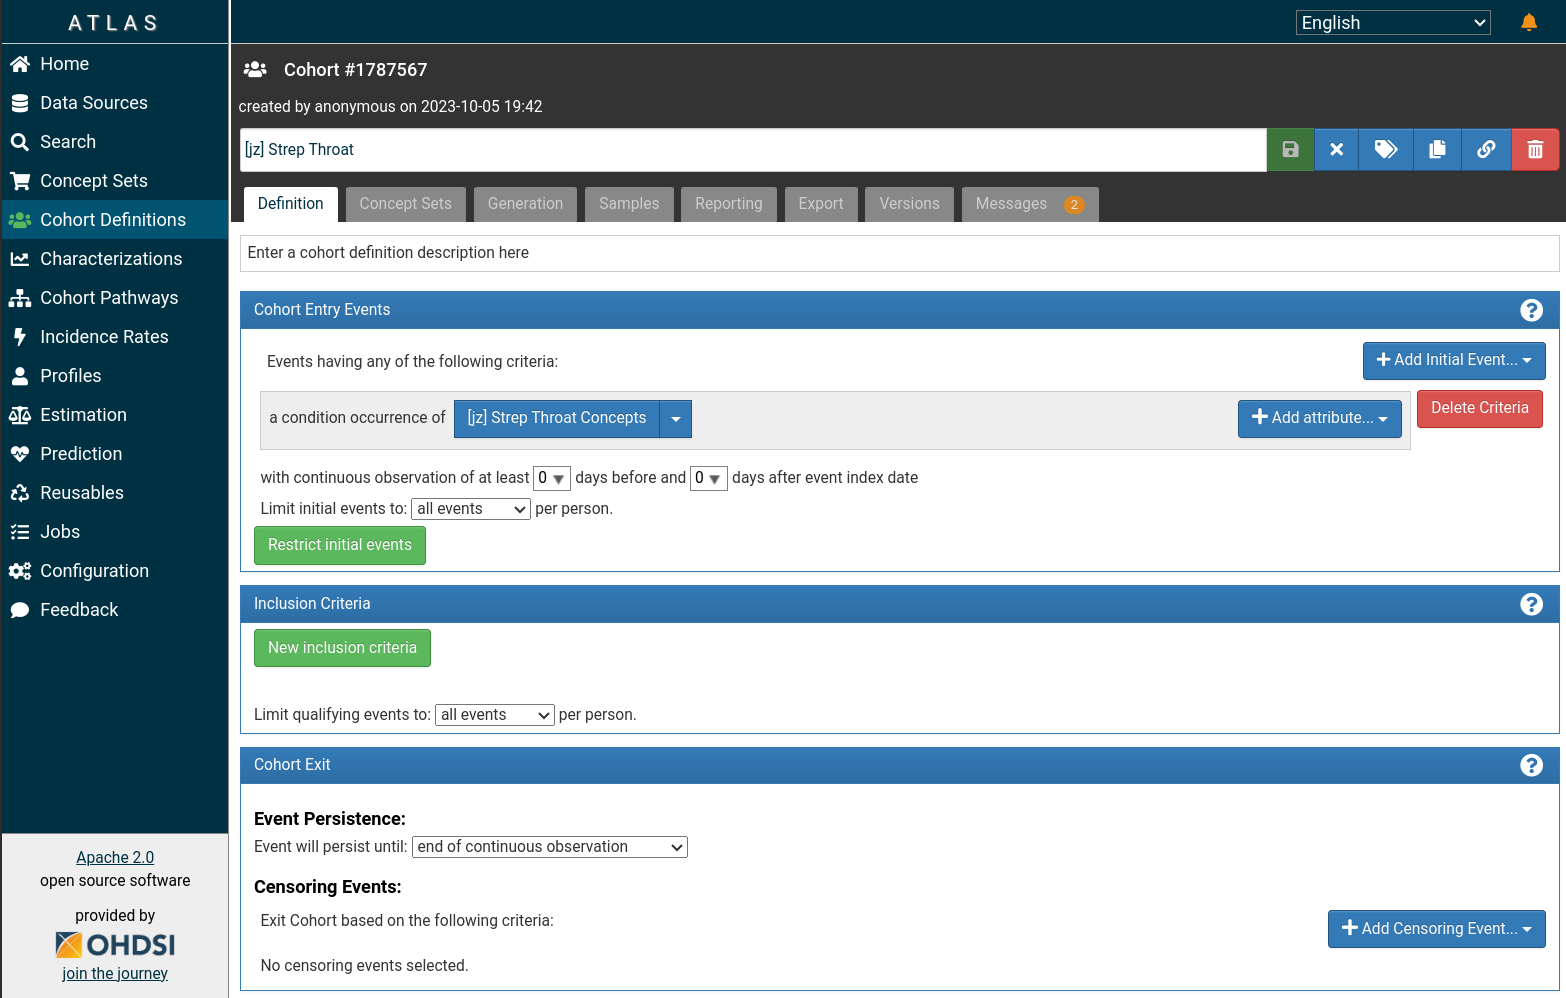
\includegraphics{./atlas_gui.png}

\subsection{Using a Cohort Definition To Build an Initial Cohort}

After having a strep throat phenotype definition defined using ATLAS, we can then execute the resulting computable phenotype definition against the \textit{Eunomia} database.

\begin{verbatim}
  using JSON3 
  using OHDSICohortExpressions

  import DBInterface as DBI

  cohort = JSON3.read("strep_throat.json")
  cohort_expression = cohort[:items][1][:expression]

  model = Model(cdm_version=v"5.3.1", cdm_schema="main",
                       vocabulary_schema="main", results_schema="main",
                       target_schema="main", target_table="cohort");

  sql = translate(cohort_expression, dialect=:sqlite, model=model, cohort_definition_id=1);

  [DBI.execute(conn, sub_query) for sub_query in split(sql, ";")[1:end-1]]
\end{verbatim}

A quick query of the cohort table (where the resulting subjects were stored) shows $\approx 1600$ from the dataset match this criteria.

TODO: Clean up the code a little nicer
TODO: Make sure the JSON3 reading of a cohort works properly

\subsection{Characterizing Patient Populations}

\begin{verbatim}
  patients = DBI.execute(conn, "SELECT subject_id AS person_id FROM cohort;") |> DF.DataFrame
\end{verbatim}

TODO: Replace this line from Jay's PR for getting cohorts

\begin{verbatim}
  patients_race = occ.GetPatientRace(patients.person_id, conn)
  patients_gender = occ.GetPatientGender(patients.person_id, conn)

  patients_age_group = occ.GetPatientAgeGroup(
    patients.person_id, 
    conn; 
    age_groupings = [[age, age + 4] for age in 0:5:119]
  )
\end{verbatim}

\subsection{Calculating Crude Prevalence Rate}

\begin{verbatim}
  import DataFrames as DF

  patients_characterized = DF.outerjoin(patients_race,
                                              patients_gender,
                                              patients_age_group;
                                              on = :person_id, 
                                              matchmissing = :equal)
  patients_characterized = patients_characterized[:, DF.Not(:person_id)]
  patient_groups = DF.groupby(patients_characterized, [:race_concept_id, :gender_concept_id, :age_group])
  patient_groups = DF.combine(patient_groups, DF.nrow => :count)
\end{verbatim}

Using this analytical approach, tabulation can be quickly conducted across patients.
Additionally, throughout the process, one can perform relevant analysis methods.
Here, we'll conduct a crude prevalence calculation across the patient cohort.

|                        Race |   Gender |   Age Group | Cohort Count | Total Count |            Prev. (%) |
| ---------------------------:| --------:| -----------:| ------------:| -----------:| --------------------:|
| $Black or African American$ | $Female$ |   $60 - 64$ |         $13$ |        $21$ | $61.904761904761905$ |
|                     $White$ |   $Male$ |   $70 - 74$ |         $68$ |        $96$ |  $70.83333333333334$ |
|                     $White$ |   $Male$ |   $45 - 49$ |         $47$ |        $74$ |  $63.51351351351351$ |
|                     $White$ | $Female$ |   $50 - 54$ |         $59$ |       $111$ | $53.153153153153156$ |
| $Black or African American$ | $Female$ |   $55 - 59$ |          $7$ |        $19$ |  $36.84210526315789$ |
|                     $White$ | $Female$ | $110 - 114$ |         $22$ |        $29$ |  $75.86206896551724$ |
|                     $White$ |   $Male$ |   $75 - 79$ |         $45$ |        $56$ |  $80.35714285714286$ |
|                     $White$ | $Female$ |   $55 - 59$ |         $62$ |        $97$ |  $63.91752577319587$ |
|                     $White$ | $Female$ |   $45 - 49$ |         $41$ |        $92$ | $44.565217391304344$ |
|                     $Asian$ | $Female$ |   $80 - 84$ |          $4$ |         $5$ |               $80.0$ |
|                     $White$ | $Female$ |   $60 - 64$ |         $88$ |       $123$ |  $71.54471544715447$ |
|                     $White$ | $Female$ |   $75 - 79$ |         $43$ |        $58$ |  $74.13793103448276$ |
|                     $White$ |   $Male$ |   $60 - 64$ |         $62$ |       $106$ | $58.490566037735846$ |
|                     $White$ | $Female$ | $100 - 104$ |         $20$ |        $29$ |  $68.96551724137932$ |
|                     $White$ |   $Male$ |   $55 - 59$ |         $61$ |       $111$ |  $54.95495495495496$ |
|                     $Asian$ |   $Male$ |   $80 - 84$ |          $6$ |        $10$ |               $60.0$ |
|                     $White$ |   $Male$ |   $50 - 54$ |         $65$ |       $119$ | $54.621848739495796$ |
| $Black or African American$ | $Female$ |   $45 - 49$ |         $10$ |        $23$ |  $43.47826086956522$ |
|       $No matching concept$ | $Female$ |   $60 - 64$ |         $29$ |        $39$ |  $74.35897435897436$ |
| $Black or African American$ |   $Male$ |   $65 - 69$ |         $12$ |        $18$ |  $66.66666666666666$ |

TODO: Fix up this table

\subsection{Summary of Results}

As seen in Table 1 and Table 2, informative results can be rapidly generated by this workflow relevant to observational health research.
Although the values shown in Table 2 are synthetic and the crude prevalence values themselves are meaningless, we can take a this approach and apply it directly to the MIMIC III dataset.
In Table 3, we can calculate across this dataset meaningful statistics that could later be further analyzed and drive further questioning (such as ...).

\section{Discussion}

\subsection{Advanced Features of the JuliaHealth Ecosystem}

    1. Modularization of code and chaining
    2. Distributed computing
    3. FunSQL back-end

\subsection{Strong Composition of Machine Learning, Differential Equations, and JuliaHealth}

\subsection{Potential Future Directions}

As shown in this work, there is a rich opportunity for the JuliaHealth organization to become a strong presence within observational health research. 
JuliaHealth is now sufficiently at a stage of maturity where potential future researchers can leverage JuliaHealth's tools to conduct further future research or build upon existing architecture to target specific needs.
Some potential future directions that can be taken are as follows.

Due to the strong composition that exists within the JuliaHealth and broader Julia ecosystem, solutions may already exist for solving various health informatics related research.
However, what has consistently been a problem within the Julia ecosystem is the lack of sufficient documentation dedicated to describing these novel compositions and their application to various endeavors.
Future efforts can be dedicated to taking existing tools and reframing them in a JuliaHealth context to assist newcomers to Julia and JuliaHealth in determining how to explore and address problems that they are interested in.

Additionally, due to the composable and modular nature of the observational health sub-ecosystem, research analyses and visualizations can be decoupled and interchanged with one another.
Whereas in other ecosystems that make technologies for tools such as dashboards tightly coupled to analytics regimens, the subecosystem is mature enough to enable new users and developers to create analytics tools that can be separately woven into more graphical user interfaces.
For example, treatment pathways is a novel observational health approach to understand and visualize the care a patient receives within a care setting.
Only a few tools exist to visualize such hidden patient narratives but with the JuliaHealth ecosystem, the possibility of making tools that can interrogate patient care pathways more deeply could be fully realized.

Furthermore, again exploiting the composition within the JuliaHealth ecosystem, as mentioned in the context of JuliaHealth and machine learning applications, future efforts could focus on developing fairness and bias auditing tools in patient datasets.
These tools could consider factors commonly explored in health equity literature like data completeness, demographic variables, and fairness algorithms. 

Moreover, there's potential to advance clinical informatics by developing a flexible clinical type system, supporting computable phenotype definitions and medical ontologies. The ecosystem can also benefit from tools to audit the fairness of phenotype definitions. Finally, as the landscape of data expands, integrating non-traditional sources like social media and environmental data into standardized patient records will be a critical frontier. In these ways, JuliaHealth is primed to drive innovation in observational health informatics, pushing the boundaries of data-driven healthcare research.


\section{Conclusion}



\section{Acknowledgements}

For this work, we would like to thank and recognize the following individuals and groups: Dr. Jon Duke and Charity Hilton for their early support, 

\section{References}

% APPENDIX
\appendix

\section{JSON Serialization of Computable Phenotype Definition}\label{appendix:json}

An example of the JSON serialization of computable phenotype definitions can be found within the paper repository here:

In particular, this example seeks to identify individuals with Type 2 Diabetes Mellitus within a given OMOP CDM.

This was generated using ATLAS Version 2.12.1 as well as 
WebAPI Version 2.12.1.
A generic definition of the schema that was created for ATLAS 2.7.1 can be explored here: https://github.com/OHDSIBr/ATLAS-JSON-Schema/tree/2.7.4

\section{PostgreSQL Serialization of Computable Phenotype Definition}\label{appendix:postgresql}

An example of a PostgreSQL SQL serialization of computable phenotype definitions can be found within the paper repository here:

In particular, this example seeks to identify individuals with Type 2 Diabetes Mellitus within a given OMOP CDM.

This was generated using ATLAS Version 2.12.1 as well as 
WebAPI Version 2.12.1.

% **************GENERATED FILE, DO NOT EDIT**************

\bibliographystyle{juliacon}
\bibliography{ref.bib}


\end{document}

% Paragraph 1: Background on observational health research

% Observational health data captures a comprehensive view of patient cohort populations, and they are often used to assess incidence rates, prevalence rates, risk factors, and prognosis associated with physical and mental health conditions and treatment interventions. By analyzing healthcare records and clinical events, observational health research can perform cohort characterization, population-estimation, and patient-level predictions to evaluate population health, target interventions and prevention measures, and ultimately transform healthcare policy.    

% However, current observational health and epidemiological surveys are limited by their data collection and administration methods, sample size representativeness, cohort phenotype definitions, and statistical/algorithmic methods to combine outside, disparate data sources. There is a need for timely, unbiased, accurate, and quality data regarding the mental illness and the ability detect and characterize trends in prevalence, severity, and the association with other chronic illnesses/morbidities. 

% This effort could help leading health officials implement better informed interventions that will increase equitable access to mental healthcare across vulnerable populations, support efforts to decrease acute mental health-related morbidities, and improve efficacy of health spending. 

% Paragraph 2: What is OHDSI + HADES R ecosystem

% Observational Health Data Sciences and Informatics (OHDSI) is a global, collaborative, interdisciplinary, and open-science network of researchers, healthcare professionals, students, patients, other individuals and organizations committed to large-scale health data analytics and generating reliable evidence, with the goal of promoting better health decisions and better care. 

% Since current observational health data sources are aggregated at different levels and cannot be generalized to the overall population, the data is often incomplete, inaccurate, and prone to issues of bias, error handling, and multidimensional complexity. The goal of OHDSI is to produce reproducible, robust, and reliable evidence by developing standardized data formats and research protocol designs to enable large-scale collaborative research and improve the transparency and scalability of observational health research. 

% The development of the Observational Medical Outcomes Partnership (OMOP) was created in 2009 to address concerns related to data type, study design, and data privacy concerns. The OMOP Common Data Model (CDM) is a "person-centered" information model with standardized relationships and structures with other event tables to create a longitudinal view of all clinical, healthcare-related events for each person. 

% OHDSI also develops open-source analytical and software tools, such as HADES and ATLAS, which features a comprehensive set of functions needed to conduct network studies from assessing demographic information to generating summary statistics and interactive dashboards. The best practices set forth by OHDSI has improved the quality and reliability of evidence in observational studies, and it improved network research study collaboration, supported large-scale analytics, and standardized data structures and medical vocabulary.  

% Health Analytics Data-to-Evidence Suite (HADES) is a collection of 20 R packages, developed by the OHDSI team, that interact directly with the OMOP CDM to support large-scale analytics, including cohort construction (CirceR, CohortGenerator), population-level estimation (CohortMethod), patient-level prediction (PatientLevelPrediction), and return statistics, figures, and tables. 

% Paragraph 3: Why tooling was needed

% Old Content

% \subsection{Tooling for Observational Health Research}

% Paragraph 1: Introduction of novel packages

% Paragraph 2: Development philosophy and algorithmic design

% \subsection{Example Use Cases}

% \subsubsection{Minimal Characterization Study}

% Paragraph 1: Condensed version of tutorial: https://juliahealth.org/OMOPCDMCohortCreator.jl/dev/tutorials/

% Paragraph 2: Example of using results (base off this paragraph): From here, the potential to calculate valuable metrics disease prevalence across niche populations is rich and opens up the possibility to do even more with these subpopulations one could generate (e.g. cross walking with survey panel data, area estimation, etc.). Furthermore, I have tested this but have not had an opportunity to write a tutorial on the matter, but these functionalities work with Distributed.jl to enable non-blocking asynchronous code execution (still working out exact approach/functionalities) to fully utilize Julia’s performance when working and transforming large amounts of data that is often found in observational studies.

% \subsubsection{Composability within Ecosystem} 

% Paragraph 1 - 2: Distributed computing + Distributed.jl (maybe with Memoization) + Light benchmarking (?)

% Paragraph 3: Support for other databases + FunSQL.jl + SQL output

% \section{Discussion}

% Paragraph 1: How it is being used

% Paragraph 2: Next steps and Future - base off of this: As I was recently funded another year to continue my health disparities research (yay!), I have great ambitions to build out observational health research capacity in JuliaHealth through avenues such as:

% Finalize a submission to JuliaCon Proceedings (need to finish writing tests across this portfolio and adding documentation in the coming weeks)
% Partnering on potentially running studies within the Julia community using these tools
% Scoping out better support for survey and panel data
% Building additional tooling around observational health research (such as determining fairness metrics, easily deployable interactive results explorers, interop with OHDSI tools, etc.)
% Lowering barrier to entry of prototyping large scale studies for researchers
